%% BioMed_Central_Tex_Template_v1.06
%%                                      %
%  bmc_article.tex            ver: 1.06 %
%                                       %

%%IMPORTANT: do not delete the first line of this template
%%It must be present to enable the BMC Submission system to
%%recognise this template!!

%%%%%%%%%%%%%%%%%%%%%%%%%%%%%%%%%%%%%%%%%
%%                                     %%
%%  LaTeX template for BioMed Central  %%
%%     journal article submissions     %%
%%                                     %%
%%          <8 June 2012>              %%
%%                                     %%
%%                                     %%
%%%%%%%%%%%%%%%%%%%%%%%%%%%%%%%%%%%%%%%%%


%%%%%%%%%%%%%%%%%%%%%%%%%%%%%%%%%%%%%%%%%%%%%%%%%%%%%%%%%%%%%%%%%%%%%
%%                                                                 %%
%% For instructions on how to fill out this Tex template           %%
%% document please refer to Readme.html and the instructions for   %%
%% authors page on the biomed central website                      %%
%% http://www.biomedcentral.com/info/authors/                      %%
%%                                                                 %%
%% Please do not use \input{...} to include other tex files.       %%
%% Submit your LaTeX manuscript as one .tex document.              %%
%%                                                                 %%
%% All additional figures and files should be attached             %%
%% separately and not embedded in the \TeX\ document itself.       %%
%%                                                                 %%
%% BioMed Central currently use the MikTex distribution of         %%
%% TeX for Windows) of TeX and LaTeX.  This is available from      %%
%% http://www.miktex.org                                           %%
%%                                                                 %%
%%%%%%%%%%%%%%%%%%%%%%%%%%%%%%%%%%%%%%%%%%%%%%%%%%%%%%%%%%%%%%%%%%%%%

%%% additional documentclass options:
%  [doublespacing]
%  [linenumbers]   - put the line numbers on margins

%%% loading packages, author definitions

%\documentclass[twocolumn]{bmcart}% uncomment this for twocolumn layout and comment line below
\documentclass[doublespacing]{bmcart}

%%% Load packages
%\usepackage{amsthm,amsmath}
%\RequirePackage{natbib}
%\RequirePackage[authoryear]{natbib}% uncomment this for author-year bibliography
%\RequirePackage{hyperref}
\usepackage[utf8]{inputenc} %unicode support
%\usepackage[applemac]{inputenc} %applemac support if unicode package fails
%\usepackage[latin1]{inputenc} %UNIX support if unicode package fails

\usepackage{lineno}
%%%%%%%%%%%%%%%%%%%%%%%%%%%%%%%%%%%%%%%%%%%%%%%%%
%%                                             %%
%%  If you wish to display your graphics for   %%
%%  your own use using includegraphic or       %%
%%  includegraphics, then comment out the      %%
%%  following two lines of code.               %%
%%  NB: These line *must* be included when     %%
%%  submitting to BMC.                         %%
%%  All figure files must be submitted as      %%
%%  separate graphics through the BMC          %%
%%  submission process, not included in the    %%
%%  submitted article.                         %%
%%                                             %%
%%%%%%%%%%%%%%%%%%%%%%%%%%%%%%%%%%%%%%%%%%%%%%%%%



%\def\includegraphic{}
%\def\includegraphics{}
\usepackage{graphicx}


%%% Put your definitions there:
\startlocaldefs
\endlocaldefs


%%% Begin ...
\begin{document}

%%% Start of article front matter
\begin{frontmatter}

\begin{fmbox}
\dochead{Research}

%%%%%%%%%%%%%%%%%%%%%%%%%%%%%%%%%%%%%%%%%%%%%%
%%                                          %%
%% Enter the title of your article here     %%
%%                                          %%
%%%%%%%%%%%%%%%%%%%%%%%%%%%%%%%%%%%%%%%%%%%%%%

\title{Controlling for off-target genetic effects using polygenic scores improves the power of genome-wide association studies}

%%%%%%%%%%%%%%%%%%%%%%%%%%%%%%%%%%%%%%%%%%%%%%
%%                                          %%
%% Enter the authors here                   %%
%%                                          %%
%% Specify information, if available,       %%
%% in the form:                             %%
%%   <key>={<id1>,<id2>}                    %%
%%   <key>=                                 %%
%% Comment or delete the keys which are     %%
%% not used. Repeat \author command as much %%
%% as required.                             %%
%%                                          %%
%%%%%%%%%%%%%%%%%%%%%%%%%%%%%%%%%%%%%%%%%%%%%%
\author[
  % noteref={n1}
  addressref={aff3}
]{\inits{DB}\fnm{Declan} \snm{Bennett}}
\author[
	addressref={aff2}
]{\inits{DM}\fnm{Derek} \snm{Morris}}

\author[
   addressref={aff1},                   % id's of addresses, e.g. {aff1,aff2}
   corref={aff1},                       % id of corresponding address, if any
 %  noteref={n1},                        % id's of article notes, if any
   email={cathal.seoighe@nuigalway.ie}   % email address
]{\inits{CS}\fnm{Cathal} \snm{Seoighe}}





%%%%%%%%%%%%%%%%%%%%%%%%%%%%%%%%%%%%%%%%%%%%%%
%%                                          %%
%% Enter the authors' addresses here        %%
%%                                          %%
%% Repeat \address commands as much as      %%
%% required.                                %%
%%                                          %%
%%%%%%%%%%%%%%%%%%%%%%%%%%%%%%%%%%%%%%%%%%%%%%

\address[id=aff1]{%                           % unique id
  \orgname{SFI Centre for Research Training in Genomics Data Science \& Discipline of Bioinformatics, School of Mathematics, Statistics and Applied Mathematics
National University of Ireland Galway}, % university, etc
  \street{University Road},                     %
  %\postcode{}                                % post or zip code
  \city{Galway},                              % city
  \cny{Ireland}                                    % country
}
\address[id=aff2]{%
 \orgname{Cognitive Genetics and Cognitive Therapy Group, Centre for Neuroimaging \& Cognitive Genomics, Discipline of Biochemistry, National University of Ireland Galway},
 \street{University Road},
 % \postcode{24105}
  \city{Galway},
  \cny{Ireland}
}
\address[id=aff3]{%                           % unique id
  \orgname{Discipline of Bioinformatics, School of Mathematics, Statistics and Applied Mathematics
National University of Ireland, Galway}, % university, etc
  \street{University Road},                     %
  %\postcode{}                                % post or zip code
  \city{Galway},                              % city
  \cny{Ireland}                                    % country
}
%%%%%%%%%%%%%%%%%%%%%%%%%%%%%%%%%%%%%%%%%%%%%%
%%                                          %%
%% Enter short notes here                   %%
%%                                          %%
%% Short notes will be after addresses      %%
%% on first page.                           %%
%%                                          %%
%%%%%%%%%%%%%%%%%%%%%%%%%%%%%%%%%%%%%%%%%%%%%%

%\begin{artnotes}
%\note{Sample of title note}     % note to the article
%\note[id=n1]{Equal contributor} % note, connected to author
%\end{artnotes}

\end{fmbox}% comment this for two column layout

%%%%%%%%%%%%%%%%%%%%%%%%%%%%%%%%%%%%%%%%%%%%%%
%%                                          %%
%% The Abstract begins here                 %%
%%                                          %%
%% Please refer to the Instructions for     %%
%% authors on http://www.biomedcentral.com  %%
%% and include the section headings         %%
%% accordingly for your article type.       %%
%%                                          %%
%%%%%%%%%%%%%%%%%%%%%%%%%%%%%%%%%%%%%%%%%%%%%%

\begin{abstractbox}

\begin{abstract} % abstract
%\parttitle{First part title} %if any
%Text for this section.

Ongoing increases in the size of human genotype and phenotype collections offer the promise of improved understanding of the genetics of complex diseases. In addition to the biological insights that can be gained from the nature of the variants that contribute to the genetic component of complex trait variability, these data have brought forward the prospect of predicting complex traits and the risk of complex genetic diseases from genotype data. Optimal realization of these objectives from the data that are becoming available requires ongoing methodological developments, designed to identify true trait-associated  variants and accurately predict phenotype from genotype. In addition to optimal accuracy, these methods must also be computationally efficient, in order to remain tractable in the context of high variant densities and very large sample sizes. Here we show that the power of linear mixed models that are in widespread use for GWAS can be increased significantly by modeling off target genetic effects using polygenic scores derived from SNPs that are not on the same chromosome as the target SNP. Applying this method to simulated and real data we found that it can result in a substantial increase in the number of variants passing genome-wide significance thresholds. This increase in power to detect trait-associated variants also translates into an increase in the accuracy with which the resulting polygenic score predicts the phenotype from genotype data. 

%\parttitle{Second part title} %if any
%Text for this section.
\end{abstract}

%%%%%%%%%%%%%%%%%%%%%%%%%%%%%%%%%%%%%%%%%%%%%%
%%                                          %%
%% The keywords begin here                  %%
%%                                          %%
%% Put each keyword in separate \kwd{}.     %%
%%                                          %%
%%%%%%%%%%%%%%%%%%%%%%%%%%%%%%%%%%%%%%%%%%%%%%

\begin{keyword}
\kwd{GWAS}
\kwd{PGS}
\kwd{Off-target effects}
\end{keyword}

% MSC classifications codes, if any
%\begin{keyword}[class=AMS]
%\kwd[Primary ]{}
%\kwd{}
%\kwd[; secondary ]{}
%\end{keyword}

\end{abstractbox}
%
%\end{fmbox}% uncomment this for twcolumn layout

\end{frontmatter}

%%%%%%%%%%%%%%%%%%%%%%%%%%%%%%%%%%%%%%%%%%%%%%
%%                                          %%
%% The Main Body begins here                %%
%%                                          %%
%% Please refer to the instructions for     %%
%% authors on:                              %%
%% http://www.biomedcentral.com/info/authors%%
%% and include the section headings         %%
%% accordingly for your article type.       %%
%%                                          %%
%% See the Results and Discussion section   %%
%% for details on how to create sub-sections%%
%%                                          %%
%% use \cite{...} to cite references        %%
%%  \cite{koon} and                         %%
%%  \cite{oreg,khar,zvai,xjon,schn,pond}    %%
%%  \nocite{smith,marg,hunn,advi,koha,mouse}%%
%%                                          %%
%%%%%%%%%%%%%%%%%%%%%%%%%%%%%%%%%%%%%%%%%%%%%%

%%%%%%%%%%%%%%%%%%%%%%%%% start of article main body
% <put your article body there>

%%%%%%%%%%%%%%%%
%% Background %%
%%

\linenumbers
\section*{Bachground}

Linear mixed effects models (LMMs) are routinely applied to detect associations between SNPs and phenotypes in genome-wide association studies (GWAS). The contribution of a given SNP to the phenotype is modelled as a fixed effect, while the contribution of all other SNPs is modelled as a random effect, with the covariance structure of this random effect corresponding to the genetic relationships between the individuals in the study. In order to avoid including the component of the genetic relatedness contributed by variants in linkage disequilibrium (LD) with the tested variant, the genetic relationship matrix (GRM) is calculated using an LD-pruned set of variants \cite{yu2006unified,emma}. Originally these methods assumed that a large number of SNPs may each make small contributions to the phenotypic variation, such that the phenotypic contribution of the genetic background could be modelled as a multivariate normal (with covariance matrix proportional to the GRM) \cite{emma, emmax,gemma,fastlmm}. Newer implementations of these models have allowed for the possibility of a combination of SNPs with effect sizes close to zero as well as some SNPs with large effect sizes. This can be done by modelling the effect sizes of background SNPs as a mixture of normal distributions, with a proportion, $p << 1$, of SNPs with large effect sizes and the remainder with effect sizes close to zero. This results in a ‘spike and slab’ mixture model for the SNP effect sizes \cite{BOLT} (the spike corresponds to a normal component with small variance and the slab corresponding to a second normal component with large variance). Implementations of these normal mixture models have been developed that can be applied to biobank-scale data \cite{boltukb}. In addition to controlling for the direct genetic effects of other SNPs on the phenotype LMM methods have also been shown to account well for subtle population structure, and cryptic relatedness between individuals in the sample population \cite{yu2006unified,emma,emmax,gemma,price2010new}.  

 \par


Various options have been explored for which SNPs to include in the calculation of the GRM \cite{yang2014advantages}. Including SNPs in LD with the target SNP results in loss of power, as the effect of the target SNP is partially accounted for by the random effect through the GRM. This has been referred to as proximal contamination \cite{listgarten2012improved}. On the other hand, including all (or most) SNPs that are not in LD with the target SNP, e.g. using a Leave One Chromosome Out (LOCO) approach, can result in dilution of the extent to which the relevant part of the genetic background is captured by the GRM. In the latter case, SNPs that are not relevant, in that they do not capture direct genetic effects or tag relevant population structure effects, effectively add noise to the GRM \cite{listgarten2012improved}. Alternatively, the GRM can be built from only the SNPs that are found using a linear model to be associated with the phenotype. Although this results in an increase in statistical power \cite{fastlmm,yang2014advantages,lippert2013benefits}, it does not fully control for population structure and is not recommended if population structure is of substantial concern \cite{BOLT,yang2014advantages}. Methods have been developed that incorporate principal components into the GRM calculation built from significant SNPs; however, most of these methods are not suited to large biobank-scale data, without access to cloud computing or large compute farms \cite{tucker2014improving,canela2018atlas}. Off-target SNPs can also be included in the statistical model as fixed effects and this is the recommended approach when there are SNPs with large effect sizes \cite{yang2014advantages}. A model fitting approach to determine which SNPs to include as fixed effects has been developed, and this also results in increased power in GWAS \cite{listgarten2012improved}.  

\par 

As the genomic architecture of complex diseases is uncovered by large biobank scale data, the application of GWAS results in a clinical setting has become extremely important \cite{tam2019benefits}, one such question is the utility of complex disease polygenic scores (PGS). PGS are constructed from weighted sums of allele dosages, with the weights corresponding to the effects size of the variants. The identification of risk variants (variants in association with a phenotype) is typically inferred from the largest available GWAS, generally a meta-analysis. The clinical potential of PGS has already been shown in complex diseases such as coronary artery disease (CAD), diabetes and cancer  \cite{khera2018genome, torkamani2018personal, yanes2020clinical}. In CAD, the identification of individuals with similar risk to those with rare high-risk monogenic variants has been reported \cite{khera2018genome}. Similarly, in breast cancer, pathogenic variants in BRCA1/2 account for 25\% of familial risk of the disease with genome wide variants accounting for a further 18\% of the risk \cite{yanes2020clinical}. European bias is a significant concern in clinical application of PGS, resulting from over-represented of individuals of European ancestry in GWAS and poor generalization of PGS when applied to individuals with genetic ancestry distinct to the population from which the score was derived \cite{lambert2019towards,duncan2019analysis}.  

\par

Here, we set out to investigate whether including an additive PGS, estimated using a LOCO scheme, as a fixed effect in a linear mixed model has the potential to improve the power of GWAS. Our hypothesis is that the contribution of background genetic variation may not be adequately captured by a random effect, with covariance proportional to the GRM. In particular, stochastic variation resulting from SNPs with relatively large contributions to phenotypic variation may be better captured by the PGS. We tested this hypothesis in two ways. Firstly, using simulated data we tested for an improvement in power and precision on the task of recovering known causal variants as a function of study size, number of causal variants and trait heritability. In addition, we applied the method to standing height data from the UK Biobank and determined the number and characteristics of additional variants that were detected. For an objective assessment of performance on real data, where the true associations are unknown, we divided the data into test and training sets and predicted the phenotype in the test set. The improved performance on the critical task of complex phenotype prediction illustrates the utility of the PGS as a means of accounting for background genetic variance.

\section*{Results}
We simulated data to evaluate the impact of including the PGS as a fixed effect in GWAS. The simulations consisted initially of a normally-distributed continuous trait in 100,000 individuals. The trait had a narrow-sense heritability ($h^2$) of 0.5 and there were 1,000 causal SNPs with normally-distributed effects on the trait (see Methods for details). We incorporated the LOCO PGS as a fixed effect in a linear mixed model using GCTA fastGWA \cite{jiang2019resource} (a method we refer to as PGS-LMM) and found a substantial improvement in power to detect the known causal SNPs (Fig 1). In 100 simulations we found that the PGS-LMM recovered, on average, 76 additional causal variants below the conventional P-value threshold of $5x10^{-8}$ compared to fastGWA (Fig 1), corresponding to relative increases in power of 17\%. The contribution to phenotype variance of off-target SNPs can also be modelled as a random effect in a linear mixed model. This approach is applied by BOLT-LMM, which uses a normal mixture random effect, with a component corresponding to SNPs with large effects; however, PGS-LMM achieved higher power than BOLT-LMM, suggesting that first calculating a PGS from an initial GWAS and including this as a fixed effect in a mixed model may provide a better means to control for off-target genetic effects (Fig 1).  \par 

To investigate whether the increased number of causal variants recovered under PGS-LMM reflected a reduction in P-values across the board or also an improvement in the ordering of the variants, when the variants are ordered by the evidence of an association with the phenotype, we calculated receiver operator characteristic (ROC) curves for the fastGWA and PGS-LMM method (i.e. fastGWA with the LOCO PGS included as a fixed effect covariate). Over 100 simulations we found that the area under the ROC curve (AUC) was always higher for PGS-LMM than for fastGWA. The difference in sensitivity as a function of specificity (Fig. 2) showed that the ordering of SNPs is significantly improved under PGS-LMM. The PGS-LMM method provided an improvement of up to 0.051 in the mean sensitivity (corresponding to a relative improvement of 8.2\% in sensitivity compared to the fastGWA method at a specificity of 0.9992).

\subsection*{Dependence on trait heritability and number of causal variants}
We simulated data over a range of values of $h^2$ and of the number of causal SNPs. As we would expect, for very low values of $h^2$ PGS-LMM offers very little improvement over fastGWA (although the proportion of causal variants detected below a p-value threshold of $5x10^{-8}$ was always greater for PGS-LMM). From a $h^2$ value of around 0.4 the proportion of the causal variants tended to be significantly greater for PGS-LMM than for fastGWA (Fig 3a). Similarly, when there was a small number of causal variants (with a fixed value of $h^2$ = 0.5), including the polygenic score as a covariate provided little advantage; however, again, the number of causal variants recovered when the PGS was included as a covariate was always greater than or equal to the number recovered when the PGS covariate was omitted. For simulations with at least 80 causal variants the proportion of causal variants correctly identified with PGS-LMM always exceeded that obtained with the fastGWA and this difference in proportions became statistically significant as the number of causal variants approached 1,000 (Fig 3b).

\subsection*{Results of simulations with variable numbers of GWAS participants}
Including the PGS as fixed effect resulted in a higher proportion of causal variants recovered across the full range of sample sizes investigated (fig 5). Even at N=10,000 there was a significant difference between the proportion of causal variants recovered with PGS-LMM over fastGWA without PGS. This is somewhat surprising given that it is assumed that large sample sizes are required for accurate phenotype prediction from PGS \cite{dudbridge2013power}. As the sample size increased, the number of variants recovered increased sharply for both models (with and without PGS), with the rate of increase in power gradually coming down as sample numbers approach 100,000. 

\subsection*{Application to UK Biobank height data} 

We assessed performance of PGS-LMM on real data using standing height of individuals of British ancestry (429,359 individuals) from the UK Biobank. The distribution of P-values obtained from the PGS-LMM was lower than that obtained using fastGWA (See Supplementary  Figure 1, Additional File 1). At a genome-wide significance level of $5x10^{-8}$ there were 127,306 and 152,626 variants that achieved significance using fastGWA and PGS-LMM, respectively. A total of 31,332 variants were identified by PGS-LMM that did not pass the significance threshold using the fastGWA approach, termed from here as PGS-LMM only variants (See Supplementary  Figure 2, Additional File 1).  These variants were significantly enriched for low ($<$ 1\%) minor allele frequency (OR=2.44; CI=2.2-2.7; P = 6x$10^{-65}$, using Fisher’s Exact test; Fig. S3 Table S1).  We performed a gene-property analysis for tissue specificity of the PGS-LMM-only variants across 53 GTEx (v8) tissue types. Muscle and skeletal tissue had the strongest, albeit modest, association (P = 0.02; Fig. S4, Table S2, Additional File 1).  

\subsection*{Application to phenotype prediction }
One way to determine objectively whether PGS-LMM outperforms fastGWA on real data is to apply both methods on the key task of phenotype prediction. We partitioned the UKB height data into an 80\%/20\% training and testing datasets and calculated the PGS scores using a partitioning and thresholding (P+T) method as well as more powerful Bayesian method to estimate the phenotype in the test dataset (see Methods for details).  In both cases PGS-LMM consistently outperformed fastGWA across all inclusion thresholds (postererior inclusion probability (PIP) \& P-value).  The maximum $R^2$ using P+T was achieved at a P value threshold of 0.05 for both the fastGWA ($R^2= 0.129$) and PGS-LMM ($R^2= 0.138$), corresponding to a relative improvement in the proportion of the phenotype explained of 7\% (Fig. 5a). The Bayesian model provided substantially better prediction of the phenotype than PRSice2 when variants below 0.4 PIP were included in the model and, again, this performance was further enhanced when the SNP effects were estimated using PGS-LMM rather than fastGWA (Fig. 5b). The maximum $R^2$ for PGS-LMM was 0.194, compared to 0.184 with fastGWA (corresponding to a relative increase of 5.4\%). Although smaller, the improvement in performance on the prediction task remained consistent when we repeated this analysis with a 20\%/80\% training-test split (Fig. S5, Additional File 1). There are three possible reasons for the improvement in prediction obtained using PGS-LMM. It could result from a larger number of SNPs passing a given threshold being used in prediction, from improvement in the ordering of SNPs, so that a better set of SNPs are being used or, lastly, from better estimates of the SNP effect sizes. To distinguish between these possibilities we repeated the prediction using the same number of SNPs for PGS-LMM and fastGWA and then for the same set of SNPs for both (see Methods for details). The performance gain was maintained when we used the same number of SNPs, but was much smaller when we used exactly the same set of SNPs (Table S3, Additional File 1). 


\section*{Discussion}
Omitting covariates that are associated with a response and independent of an effect of interest can result in a reduction in the efficiency of the estimation of the effect of interest \cite{neuhaus1998estimation}. Complex traits are associated with the genotype of many loci across the genome, but the effects of the off-target SNPs are frequently not explicitly modelled in GWAS and, instead tests of association are performed for one target SNP at a time. We evaluated a simple two-stage approach to accounting for off-target genetic effects that consists of performing an initial GWAS and using the summary statistics to calculate a polygenic score and then including the polygenic score, derived from SNPs not on the same chromosome as the target SNP, as a fixed effect in a second round of association testing. We found that this led to a substantial improvement in GWAS power using simulated data. A popular approach to account for the effects of off-target SNPs is to make use of a mixture distribution for the random effect in a linear mixed model, with a component with large variance corresponding to off-target SNPs with large effect sizes. This approach is implemented in BOLT-LMM \cite{BOLT}. However, PGS-LMM had higher power in simulations than BOLT-LMM, suggesting that incorporating the PGS as a fixed effect in a linear model offers a better alternative for accounting for off-target genetic effects. It is also possible to include the LOCO PGS as a fixed effect with BOLT-LMM. In this case the effects of off-target SNPs are modelled both as a fixed and as a random effect. We found that this offered a small further improvement over fastGWA with the LOCO PGS (which we have referred to as Bolt PGS-LMM; Fig S6). However, this improvement comes at a substantial cost, as fastGWA is much more computationally efficient than BOLT-LMM \cite{jiang2019resource}. 

The increase in power with PGS-LMM was largest for simulated phenotypes with high heritability and a large number of causal variants (Fig. 3b). In these cases the many off-target SNPs collectively explain a substantial proportion of the phenotypic variance and summarizing the contribution of these off-target SNPs to the phenotype via the LOCO PGS is likely to result in a better estimate of the effect of the target SNP and its standard error. The boost in performance derived from including the LOCO PGS as a fixed effect was evident even for relatively small study sizes. Across all the simulation parameters we investigated, the performance of the PGS-LMM was never worse than fastGWA without the LOCO PGS. 

We also applied the method to real data (standing height in individuals of British ancestry in the UK Biobank). Height was chosen as there have been over 3,000 near independent variants associated with height explaining 0.483 of the phenotypic variance. Heritability is often estimated to be as high as 80\%. Although GWAS can only give us insight into $h^2$, the additive component of heritability, estimates of $h^2$ for height range from 0.3 for high quality common variants up to 0.88 in monozygotic twins for all SNPs \cite{yengo2018meta,hou2019accurate,nolte2017comparison}. Consistent with the simulation results, we found nearly 20\% more associated variants using the PGS-LMM, including a large number of variants (31,332) that were significant using PGS-LMM, but not using fastGWA (a much smaller set of 6,012 SNPs were identified as significant by fastGWA but not PGS-LMM; Fig S2). The newly identified variants are enriched for rare variants while common variants were depleted. The PGS-LMM identified variants were associated with expression in skeletal and muscle tissue consistent with PGS-LMM identifying additional true causal variants over fastGWA.  

The $h^2$ estimate in the simulations corresponds to the combined additive contribution to the variance of the causal SNPs; however, when we apply GWAS methods to the simulated data we do not recover all of the associated SNPs and, consequently, the estimated SNP heritabilities tends to be lower than the simulated values. For example, the simulations that were the basis of Figure 1 used $h^2 = 0.5$, but the mean estimated $h^2$ for these simulations was 0.41. This has implications for the interpretation of Figure 3a, which shows the relationship between simulated $h^2$ and power, rather than the estimated $h^2$.  Within UK Biobank, standing height has the highest estimated SNP $h^2$, at 0.52 \cite{jiang2019resource}.  PGS-LMM offers improvement over fastGWA so at higher values of $h^2$, we can expect it to yield more independent association signals for other traits such as weight, bone mineral density, baldness and platelet count that all have estimated $h^2 > 0.2$ in UK Biobank \cite{jiang2019resource}. These are traits with high heritabilities that can be easily measured in large population-based cohorts, which has enabled GWAS to already detect many association signals. Some diseases have equally high heritability, e.g., type 1 diabetes, schizophrenia and Alzheimer’s disease, but do not yet have sample sizes on the same scale as height. As this changes and statistical power of GWAS of these diseases increases, inclusion of the PGS as a fixed effect in GWAS may prove useful for identifying additional risk loci for them over and above conventional GWAS analysis. 

%PGS-LMM’s ability to detect associations with variants of lower allele frequency may also result in better performance (in terms of numbers of lead SNPs detected or accuracy of PGS) for certain traits and disorders. Such phenotypes, in comparison to hundreds of others, already have been demonstrated to have either higher proportions of rare lead SNPs (e.g. nutritional traits) or have rare lead SNPs with higher effect sizes (e.g. cognitive traits and psychiatric disorders) \cite{watanabe2019global}. 

The use of polygenic scores to contribute to phenotype prediction from genotype is an increasingly important application of the results of GWAS \cite{martin2019predicting}. Recent work has shown that PGS can identify sizeable proportions of a population with 3-times greater risk for CAD, type II diabetes (T2D), arterial fibrillation (AF), inflammatory bowel disease (IBD) and breast cancer \cite{khera2018genome}. A separate study using the FinnGen dataset compared the overall lifetime risk in coronary heart disease (CHD), T2D, AF, breast cancer and prostate cancer between individuals having an average PGS and having a high PGS score. They report that having a high PGS results in 21\% to 38\% increase in overall lifetime risk with age of onset 4 to 9 years earlier than the average cohort \cite{mars2020polygenic}. Prophylactic interventions can reduce both the physical and economic stress on health systems by entering individuals on measures to prevent and manage disease earlier. PGS when used to target individuals with high efficacy of treatment can also reduce the numbers of individuals to treat \cite{gibson2019utilization}. Although having a high PGS for a disease is not akin to a diagnosis, it can guide individuals to limit their exposure to other risk factors. Performing GWAS on a subset of samples and predicting on the remainder, we observed a consistent improvement in accuracy of the prediction of standing height in UK Biobank with PGS-LMM compared to fastGWA. Although there are many caveats surrounding the prediction of complex phenotypes, particularly clinical phenotypes \cite{duncan2019analysis}, accurate prediction of disease susceptibility can have profound implications for disease management and prevention. Our results suggest that incorporating PGS into the GWAS before recalculating PGS or otherwise predicting the phenotype or disease risk leads to improved performance on this crucial task.


\section*{Conclusion}

The tasks of detecting trait-associated variants and predicting the trait in a new sample from the summary statistics of these variants are closely intertwined. Improved performance on the trait-association task can result in more associated variants and better estimates of their effect sizes, resulting in improvement on the prediction task. On the other hand, improved methods for phenotype prediction can help to control for off-target effects in methods that identify the trait-associated variants and their effects. The method that we have explored here consists of incorporating a LOCO PGS as a fixed-effect covariate to control for these off-target effects; however, any method for phenotype prediction could play this role, once its application is restricted to variants that are not linked to the target SNP. We show here that incorporating the PGS as a fixed-effect covariate results in increased power to detect trait-associated variants in GWAS. The resulting trait-associated variants and effect size estimates lead to an improvement in the PGS, as illustrated by improved performance in the task of predicting the phenotype in a test dataset. Polygenic scores have already been shown to have clinical potential across several different traits such as CAD, T2D, Alzheimer's disease and cancer \cite{lambert2019towards}. Although sophisticated methods exist for controlling off-target genetic effects none are applicable to large scale datasets, we have shown in this work that inclusion of a simple LOCO PGS can account for these effects. This boost in power of the GWAS in turn led to an improvement in phenotype prediction. As the prediction of complex phenotypes from genotype data becomes more widespread, it is important that the underlying summary statistics from which they calculated are well estimated, with all easily identified sources of variation taken into account.
 
\section*{Methods}
\subsection*{Simulations} 

To limit the effects of population stratification only individuals that reported white British ancestry (data field 21000; code 1001) were included in all analyses. The genotype data for the simulation analysis was restricted to directly genotyped variants with minor allele frequency (MAF) greater than 0.005\%. Variants with genotype missingness greater than 2\% and failed Hardy-Weinberg equilibrium at p=0.0001 were excluded. To compute the genetic relationship matrix (GRM), a set of variants was extracted with MAF greater than 0.25\%, HWE at p=0.0005 and a genotype missingness rate of 2\%. The GRM set was further restricted by elimination of variants with an $R^2$ greater than 0.1 in a 200 variant sliding window of size 500. All genotype QC is implemented in plink2 \cite{chang2015second}. To reduce the computation time the GRM is calculation is partitioned into 250 parts using GCTAs `make-grm-part' flag. The GRM is transformed to a sparse matrix by removing sample pairs with an estimated relatedness of 0.05. To account for population structure in the association studies, principal component analysis (PCA) was performed on the set of GRM variants using plink2. The simulated traits with varying number of causal variants, narrow-sense heritability and sample size were generated using the GCTA software suite \cite{yang2011gcta}. The simulation analyses consisted of 3 studies 1), 100 rounds of $h^2$=50\% with 1000 randomly drawn causal loci and a sample size of 100,000 2), 100 rounds of 1000 fixed causal loci with varying degrees of heritability and a sample size of 100,000 and 3), varying the sample size (10,000-180,000, incrementing in 10K) with 1000 fixed causal loci and $h^2$ of 50\%. The candidate causal loci and samples were drawn at random. Association testing was performed using fastGWA with 10 PCs and assessment centre as fixed covariates. Leave-one-chromosome-out (LOCO) analysis was performed for generation of PGS fixed effects. For example, to test variants on chromosome 1 for association with the phenotype, a PGS is calculated using chromosomes 2-22. The PGS were calculated using PRSice2 (version 2.2.12 (2020-02-20))\cite{choi2019prsice}. To decrease computation time, resources and reduce the likelihood of overfitting a p-value threshold of 5e-05 was chosen a priori for the LOCO PGS calculation. Association testing was then performed using fastGWA in a chromosome-wise manner with the inclusion of the corresponding LOCO PGS fixed effect. To assess the sensitivity and specificity of the simulations, the pROC R package was used to generate receiver operating characteristic (ROC) curves \cite{robin2011proc}. For the 100 simulations in simulation study 1, BOLT-LMM association testing was also performed using the same genotypic data for association testing and GRM calculation as the fastGWA analysis with and without the inclusion of the LOCO PGS fixed effect.    

\subsection*{Application to the UK biobank data} 
\par
Autosomal genotype data was cleaned using MAF of 0.1\%, SNP-missingness of 0.02 and sample-missingness cut-off of 10\% and imputation quality thresholds of 0.8. Variants that failed HWE testing at p=5x10-7 we excluded from subsequent analysis. The total number of variants remaining after filtering was 9,156,362. The GRM is calculated using a set of LD-pruned variants with a MAF of 0.01, window size of 1000, $R^2$ of 0.9 and 100 variants window shift. This left a total of 1,326,927 to be used in the calculation of the sparse GRM using the same methods described for the simulation analysis. The PGS-LOCO was generated as described in the simulation study. The association between standing height (UKB data-field 50) and genotype was performed using the fastGWA method (GCTA version 1.93.0 beta) \cite{jiang2019resource}. Batch number, sex, age, assessment centre and 10 PCs were included as covariates. 

\subsection*{Gene-property analysis}

To test whether the PGS-LMM only variants had an association with tissue specific expression from the GTEx data, gene-property analysis was performed using the SNP2GENE functionality of the FUMA web platform \cite{watanabe2017functional}. Briefly, FUMA using MAGMA \cite{de2015magma}, maps variants to genes assigning a p-value based gene score. The Z-transformed gene scores are then modelled along with the log2 RPKM average expression in the tissue of interest, log2 RPKM of average expression across all tissues and technical confounders. To test for a positive relationship a one-sided test is then performed.  

\subsection*{Prediction}
For testing the improvement in height prediction, the UK Biobank data was partitioned into 80/20 and an independent 20/80 out-of-sample training and test using a set of 2.8 million variants (defined in the SBayesR section). We sought two PGS strategies, pruning and thresholding (P+T) and a Bayesian method (SBayesR), to test for improvement in prediction. Both methods followed the same PGS-LMM procedure in the training set and prediction in the out-of-sample except for the Bayesian method, SBayesR, which replaces PRSice in the PGS-LMM. The PGS-LMM method was applied to both the 80\% and 20\% training data. \par

For the P+T method, PGS scores were calculated in the out-of-sample set using p-values thresholds (0.001, 0.05, 0.1, 0.2, 0.3, 0.4, 0.5, 1) and model fit assessed using simple linear models. SBayesR replaces the P+T method with a more sophisticated Bayesian methods that account for the underlying genetic architecture to estimate the true effect size \cite{lloyd2019improved}. SBayesR requires the use of LD matrices with shrunk off diagonals. For computational efficiency, the shrunk LD matrix is transformed to a sparse matrix. Precomputed LD matrices for 2.8 million high-confidence UK biobank variants were downloaded from the Zenodo public repository (10.5281/zenodo.3375373). To limit the effect of overfitting, we excluded variants with a posterior inclusion probability (PIP) score of less 0.2 in the PGS-LOCO calculation. As SBayesR uses Bayesian inference to estimate the true effect sizes, Plink2 was used to extract the PGS-LOCO score from the genotype data before association testing with fastGWA. SbayesR was then applied once more on the PGS-LMM summary statistics over a range of PIP scores. \par

To assess whether the prediction performance is driven by p value or accurate estimation of effect sizes the top 74,000 non-linked sites were extracted for both the fastGWA and PGS-LMM summary statistics and P+T prediction was performed using the fixed number of variants. We chose 74,000 as it fell in the range of the number of top sites that maximise the $R^2$ value for PGS-LMM and fastGWA. 




%%%%%%%%%%%%%%%%%%%%%%%%%%%%%%%%%%%%%%%%%%%%%%
%%                                          %%
%% Backmatter begins here                   %%
%%                                          %%
%%%%%%%%%%%%%%%%%%%%%%%%%%%%%%%%%%%%%%%%%%%%%%

\begin{backmatter}

\section*{Competing interests}
  The authors declare that they have no competing interests.

\section*{Author's contributions}
    Text for this section \ldots

\section*{Acknowledgements}
  This research has been conducted using the UK Biobank Resource under Application Number 23739
%%%%%%%%%%%%%%%%%%%%%%%%%%%%%%%%%%%%%%%%%%%%%%%%%%%%%%%%%%%%%
%%                  The Bibliography                       %%
%%                                                         %%
%%  Bmc_mathpys.bst  will be used to                       %%
%%  create a .BBL file for submission.                     %%
%%  After submission of the .TEX file,                     %%
%%  you will be prompted to submit your .BBL file.         %%
%%                                                         %%
%%                                                         %%
%%  Note that the displayed Bibliography will not          %%
%%  necessarily be rendered by Latex exactly as specified  %%
%%  in the online Instructions for Authors.                %%
%%                                                         %%
%%%%%%%%%%%%%%%%%%%%%%%%%%%%%%%%%%%%%%%%%%%%%%%%%%%%%%%%%%%%%

% if your bibliography is in bibtex format, use those commands:
\bibliographystyle{bmc-mathphys} % Style BST file (bmc-mathphys, vancouver, spbasic).
\bibliography{PGS_LMM}      % Bibliography file (usually '*.bib' )
% for author-year bibliography (bmc-mathphys or spbasic)
% a) write to bib file (bmc-mathphys only)
% @settings{label, options="nameyear"}
% b) uncomment next line
%\nocite{label}

% or include bibliography directly:
% \begin{thebibliography}
% \bibitem{b1}
% \end{thebibliography}

%%%%%%%%%%%%%%%%%%%%%%%%%%%%%%%%%%%
%%                               %%
%% Figures                       %%
%%                               %%
%% NB: this is for captions and  %%
%% Titles. All graphics must be  %%
%% submitted separately and NOT  %%
%% included in the Tex document  %%
%%                               %%
%%%%%%%%%%%%%%%%%%%%%%%%%%%%%%%%%%%

%%
%% Do not use \listoffigures as most will included as separate files

\section*{Figures}
  \begin{figure}[h!]
  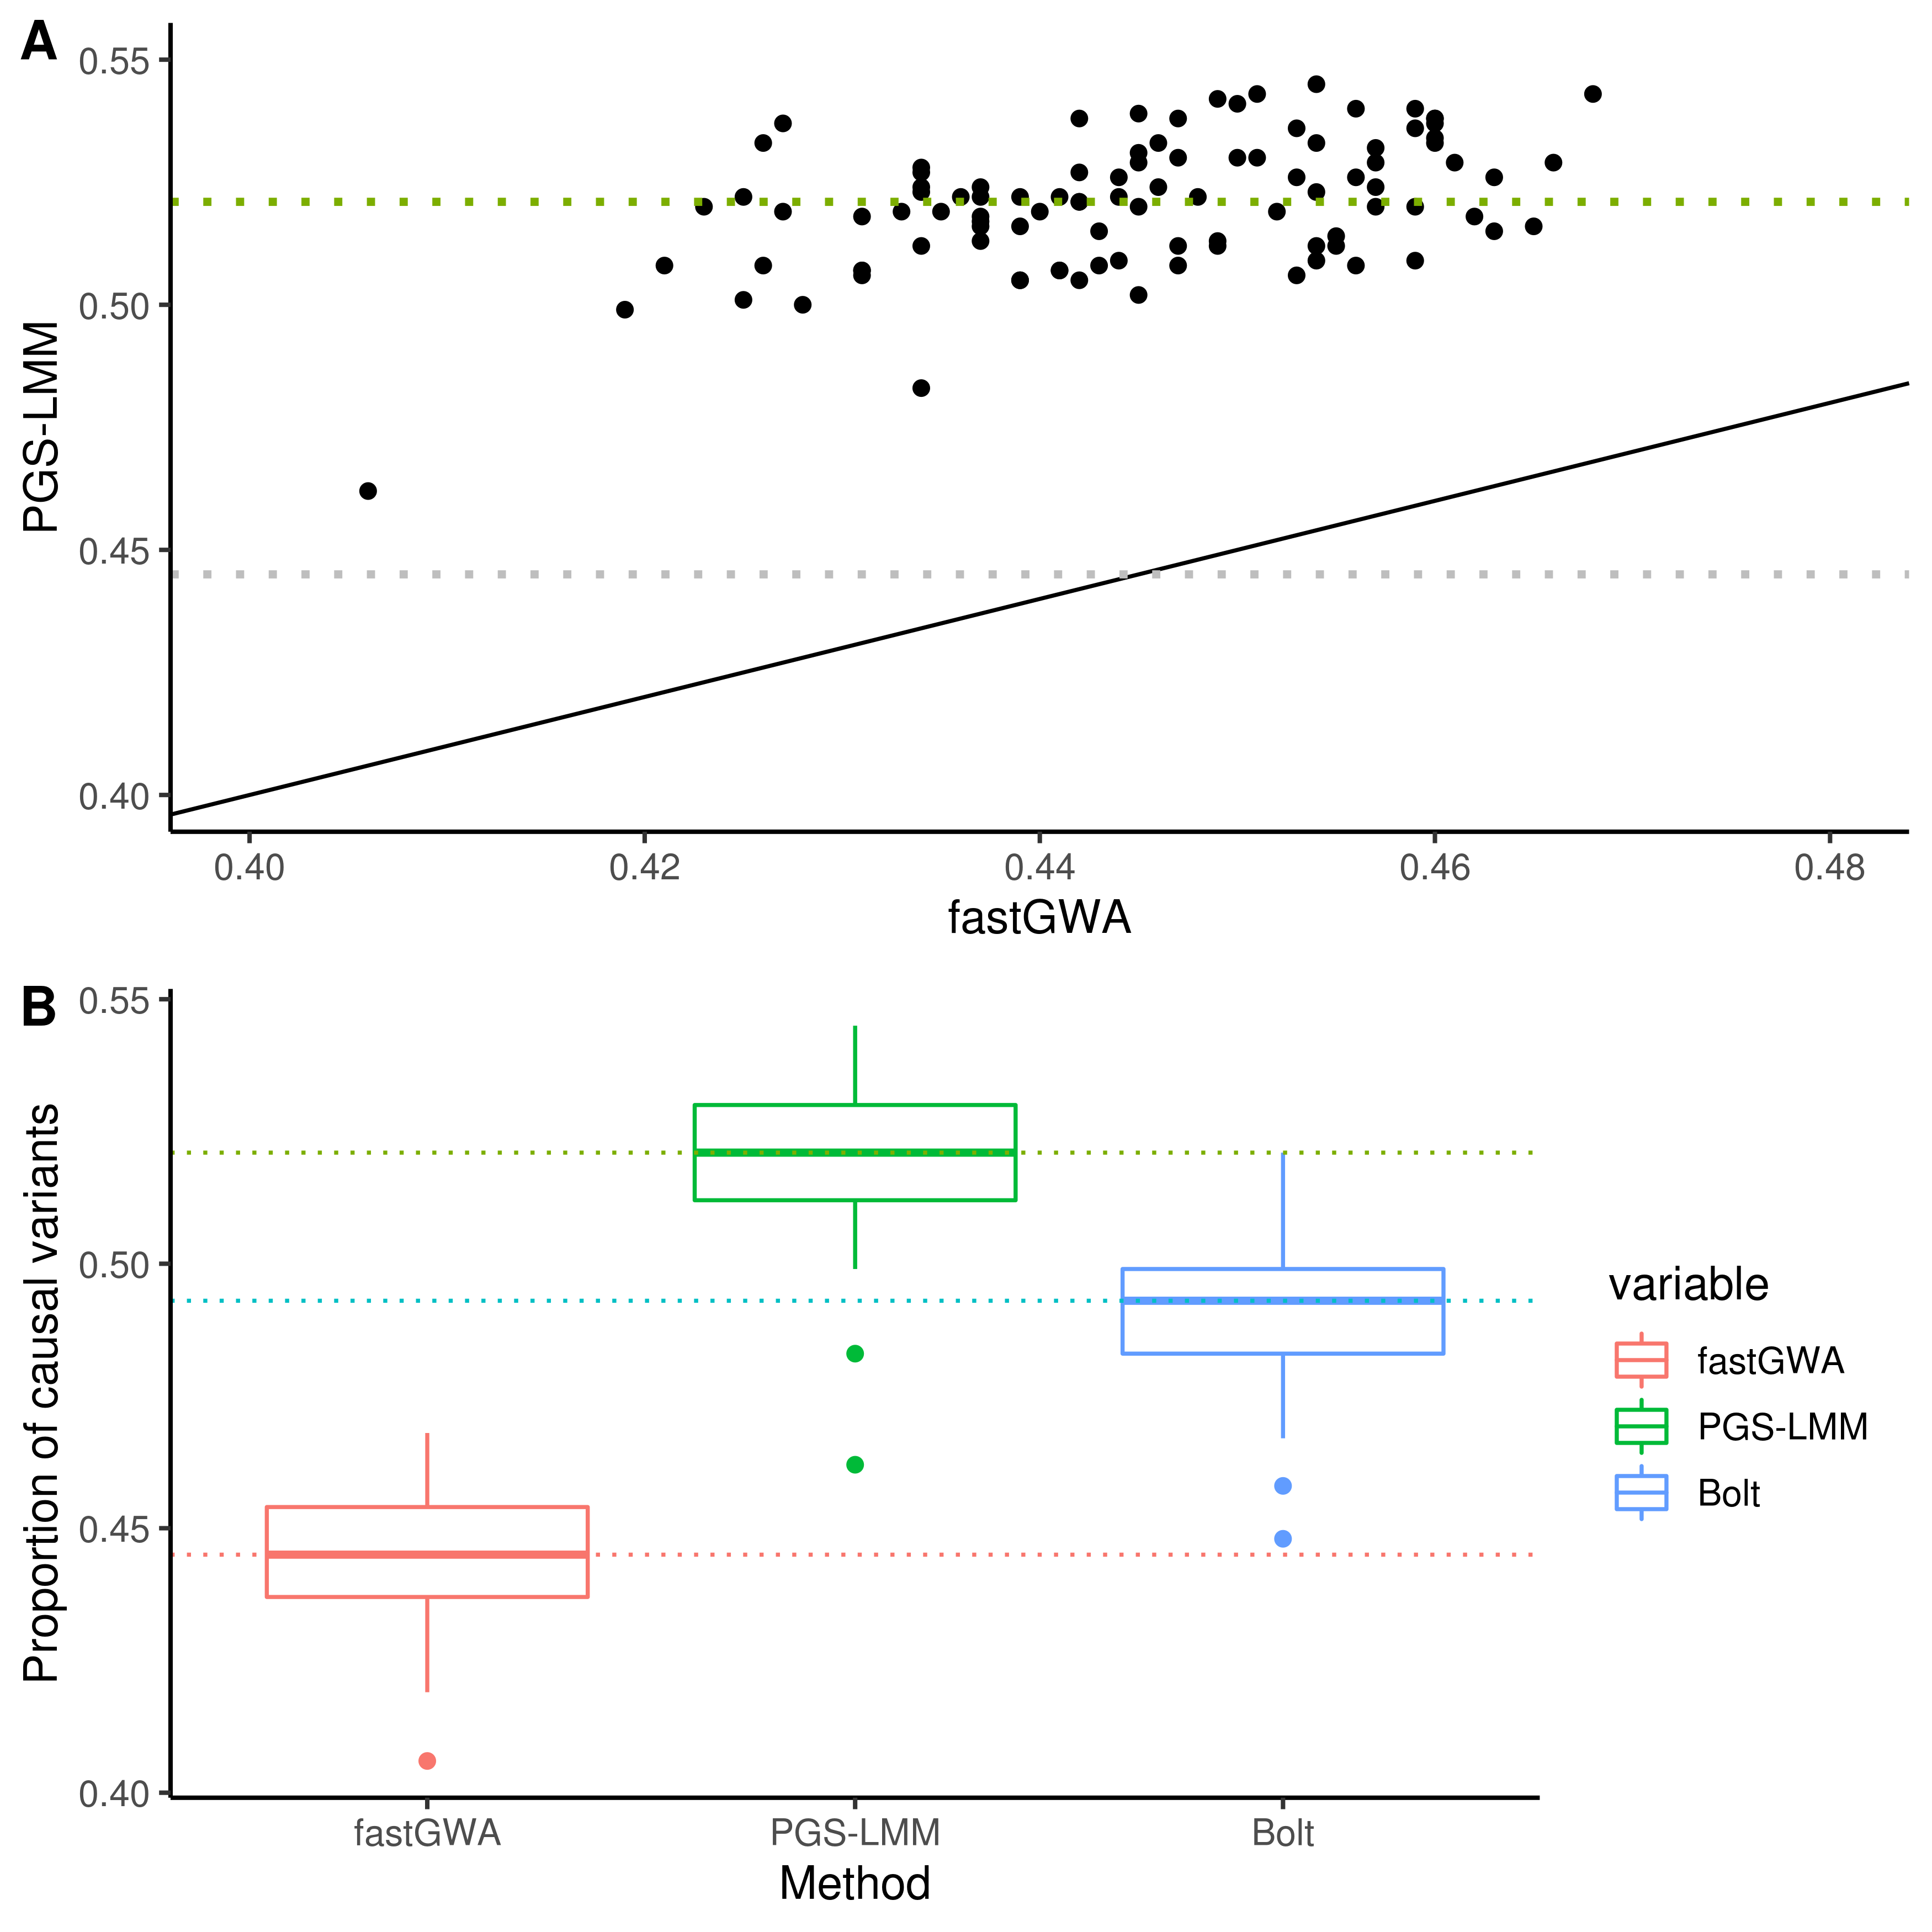
\includegraphics[width=0.85\textwidth]{images/Fig1.png}
  \caption{\csentence{Recovery of causal variants in fixed simulations.}
       (A) Scatterplot showing proportion of causal variants with P-values below a threshold of $5x10^{-8}$ in 100 simulations using the PGS-LMM (y-axis) and fastGWA (x-axis) methods. The upper and lower horizontal lines show the median number of causal variants recovered with the PGS-LMM and fastGWA methods, respectively.The black line represents the line through the origin with slope 1. (B) Proportion of causal variants identified by fastGWA, PGS-LMM and BOLT-LMM.}
      \end{figure}

\begin{figure}[h!]
	\includegraphics[width=0.85\textwidth]{images/Fig2.png}
  \caption{\csentence{Sensitivity analysis.}
      Difference in sensitivity (between the PGS-LMM and fastGWA methods) as a function of specificity. The red line shows the mean difference over all simulations.}
      \end{figure}

\begin{figure}[h!]
  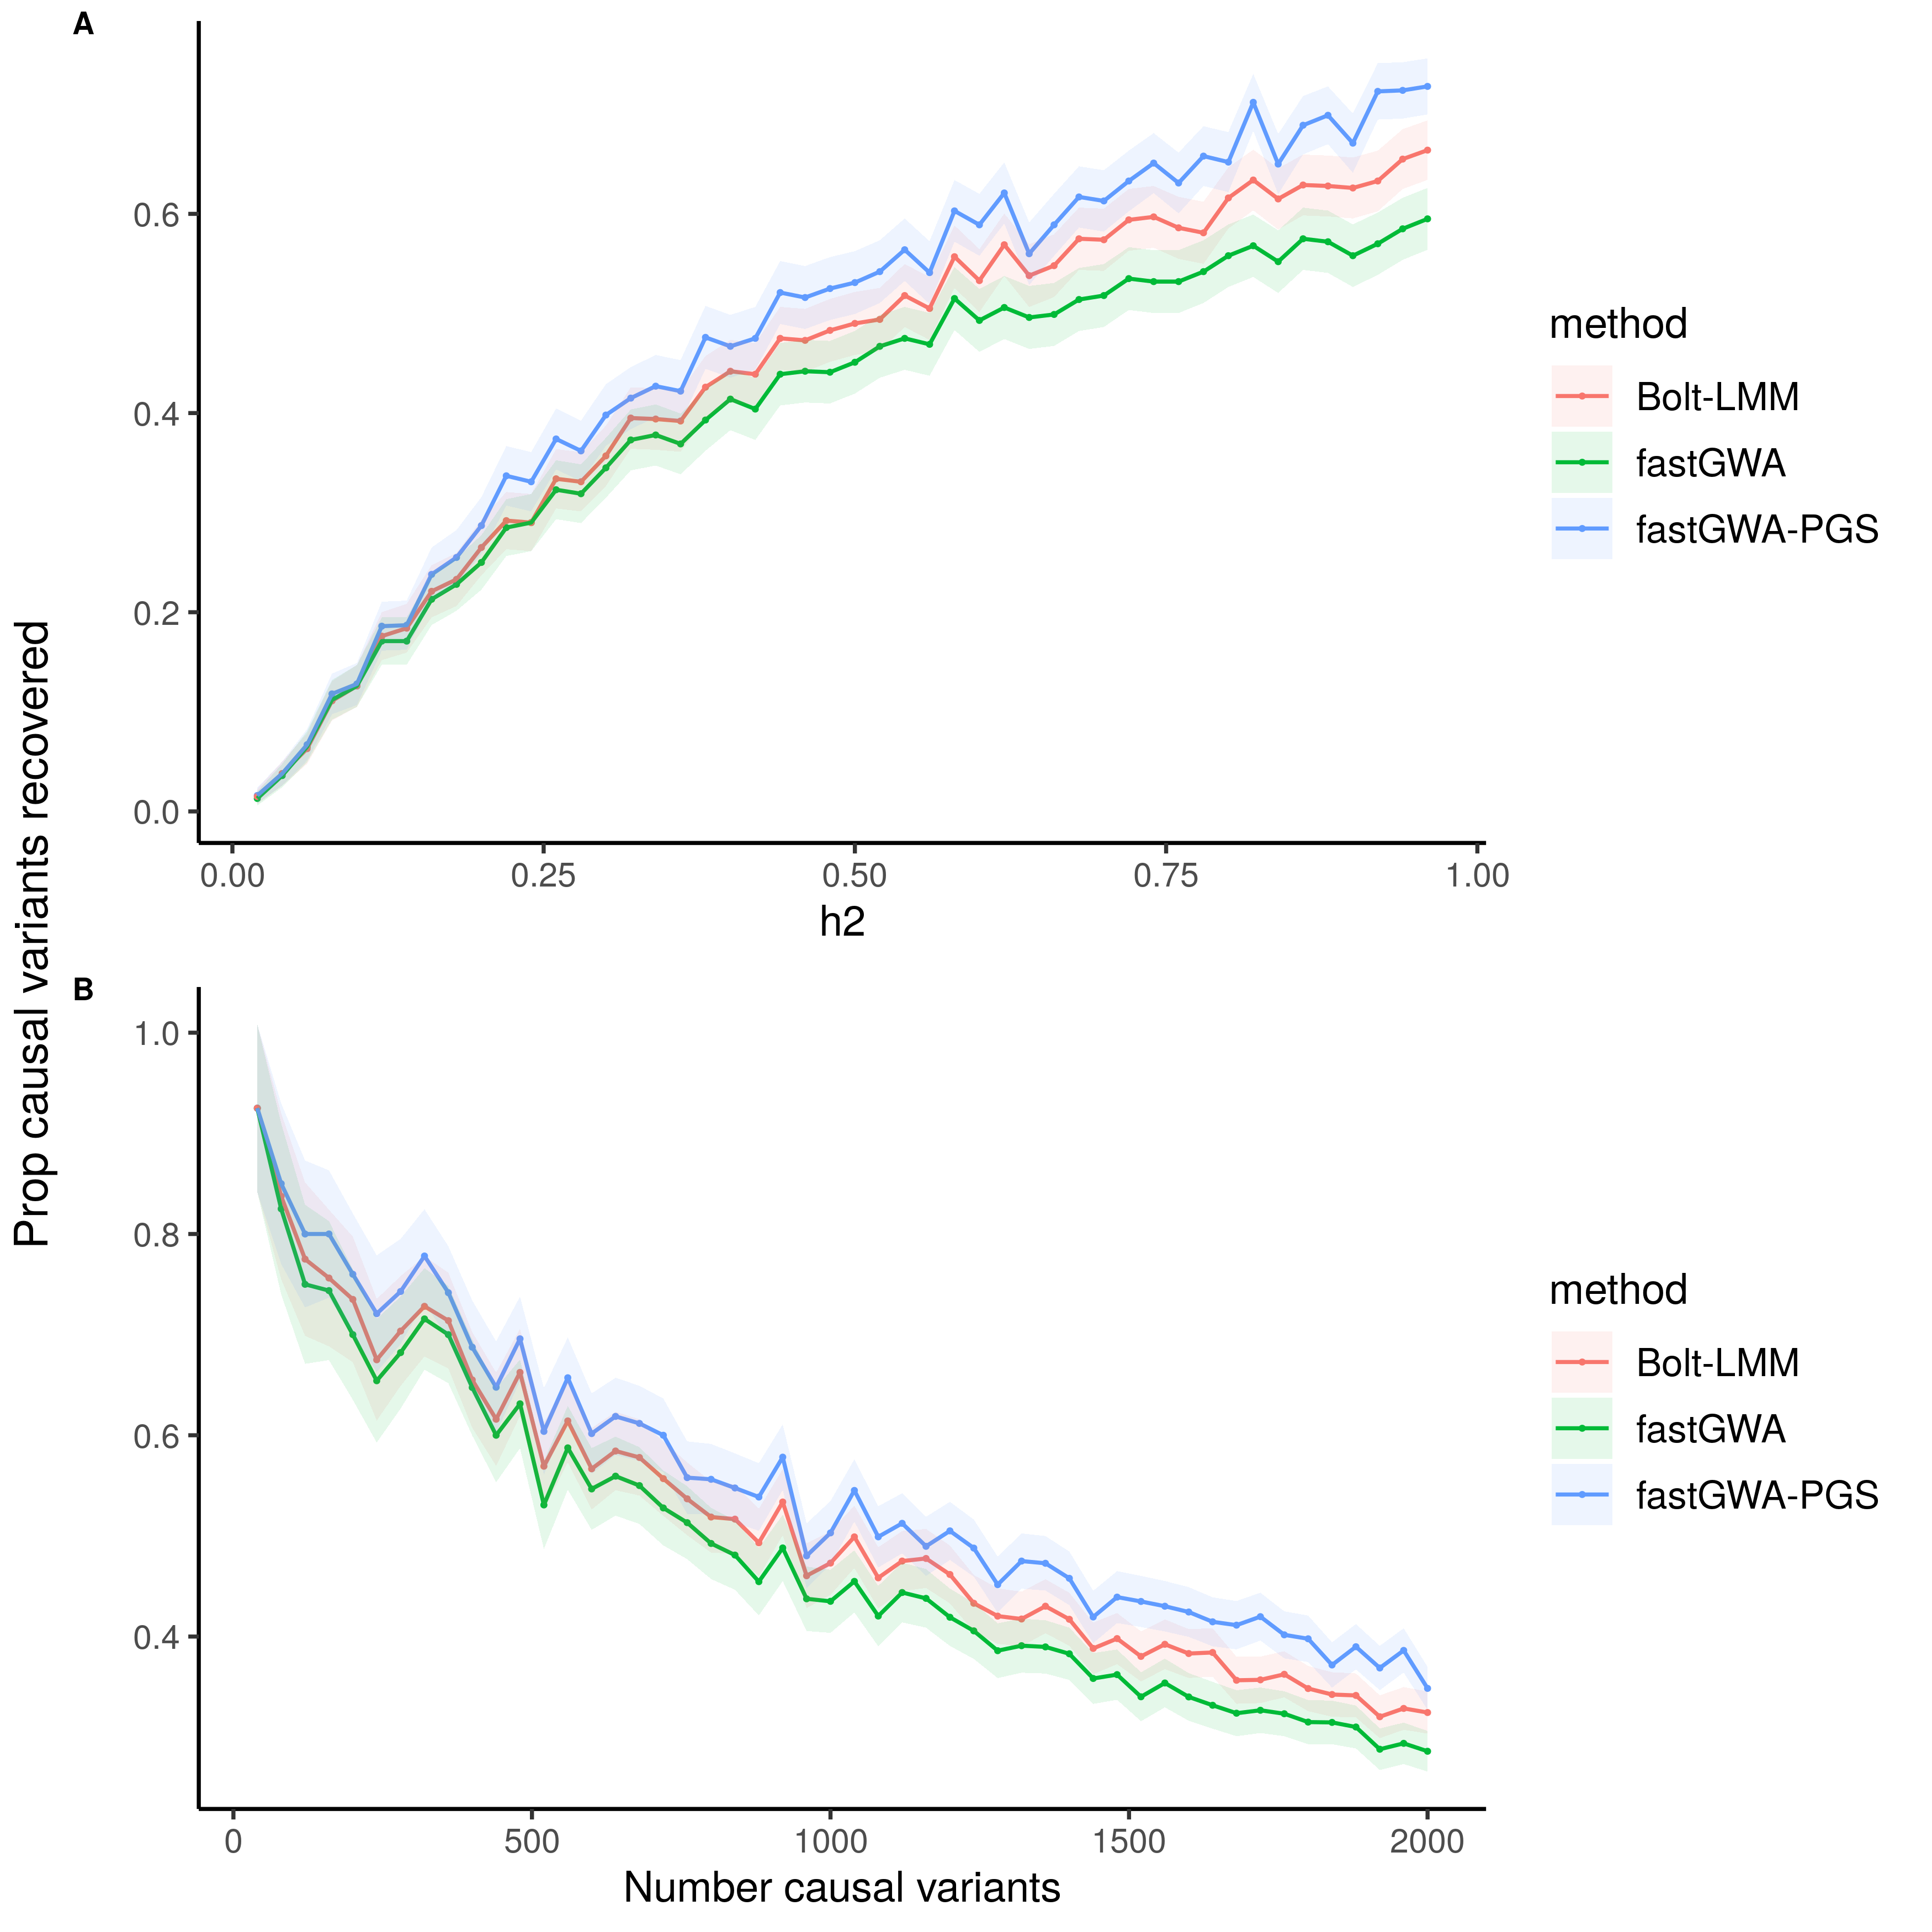
\includegraphics[width=0.85\textwidth]{images/Fig3.png}

  \caption{\csentence{Recovery of causal variants varying parameters.}
      Proportion of causal variants identified as a function of (a) the narrow-sense heritability of the simulated trait and (b) the number of causal variants.}
      \end{figure}

\begin{figure}[h!]
  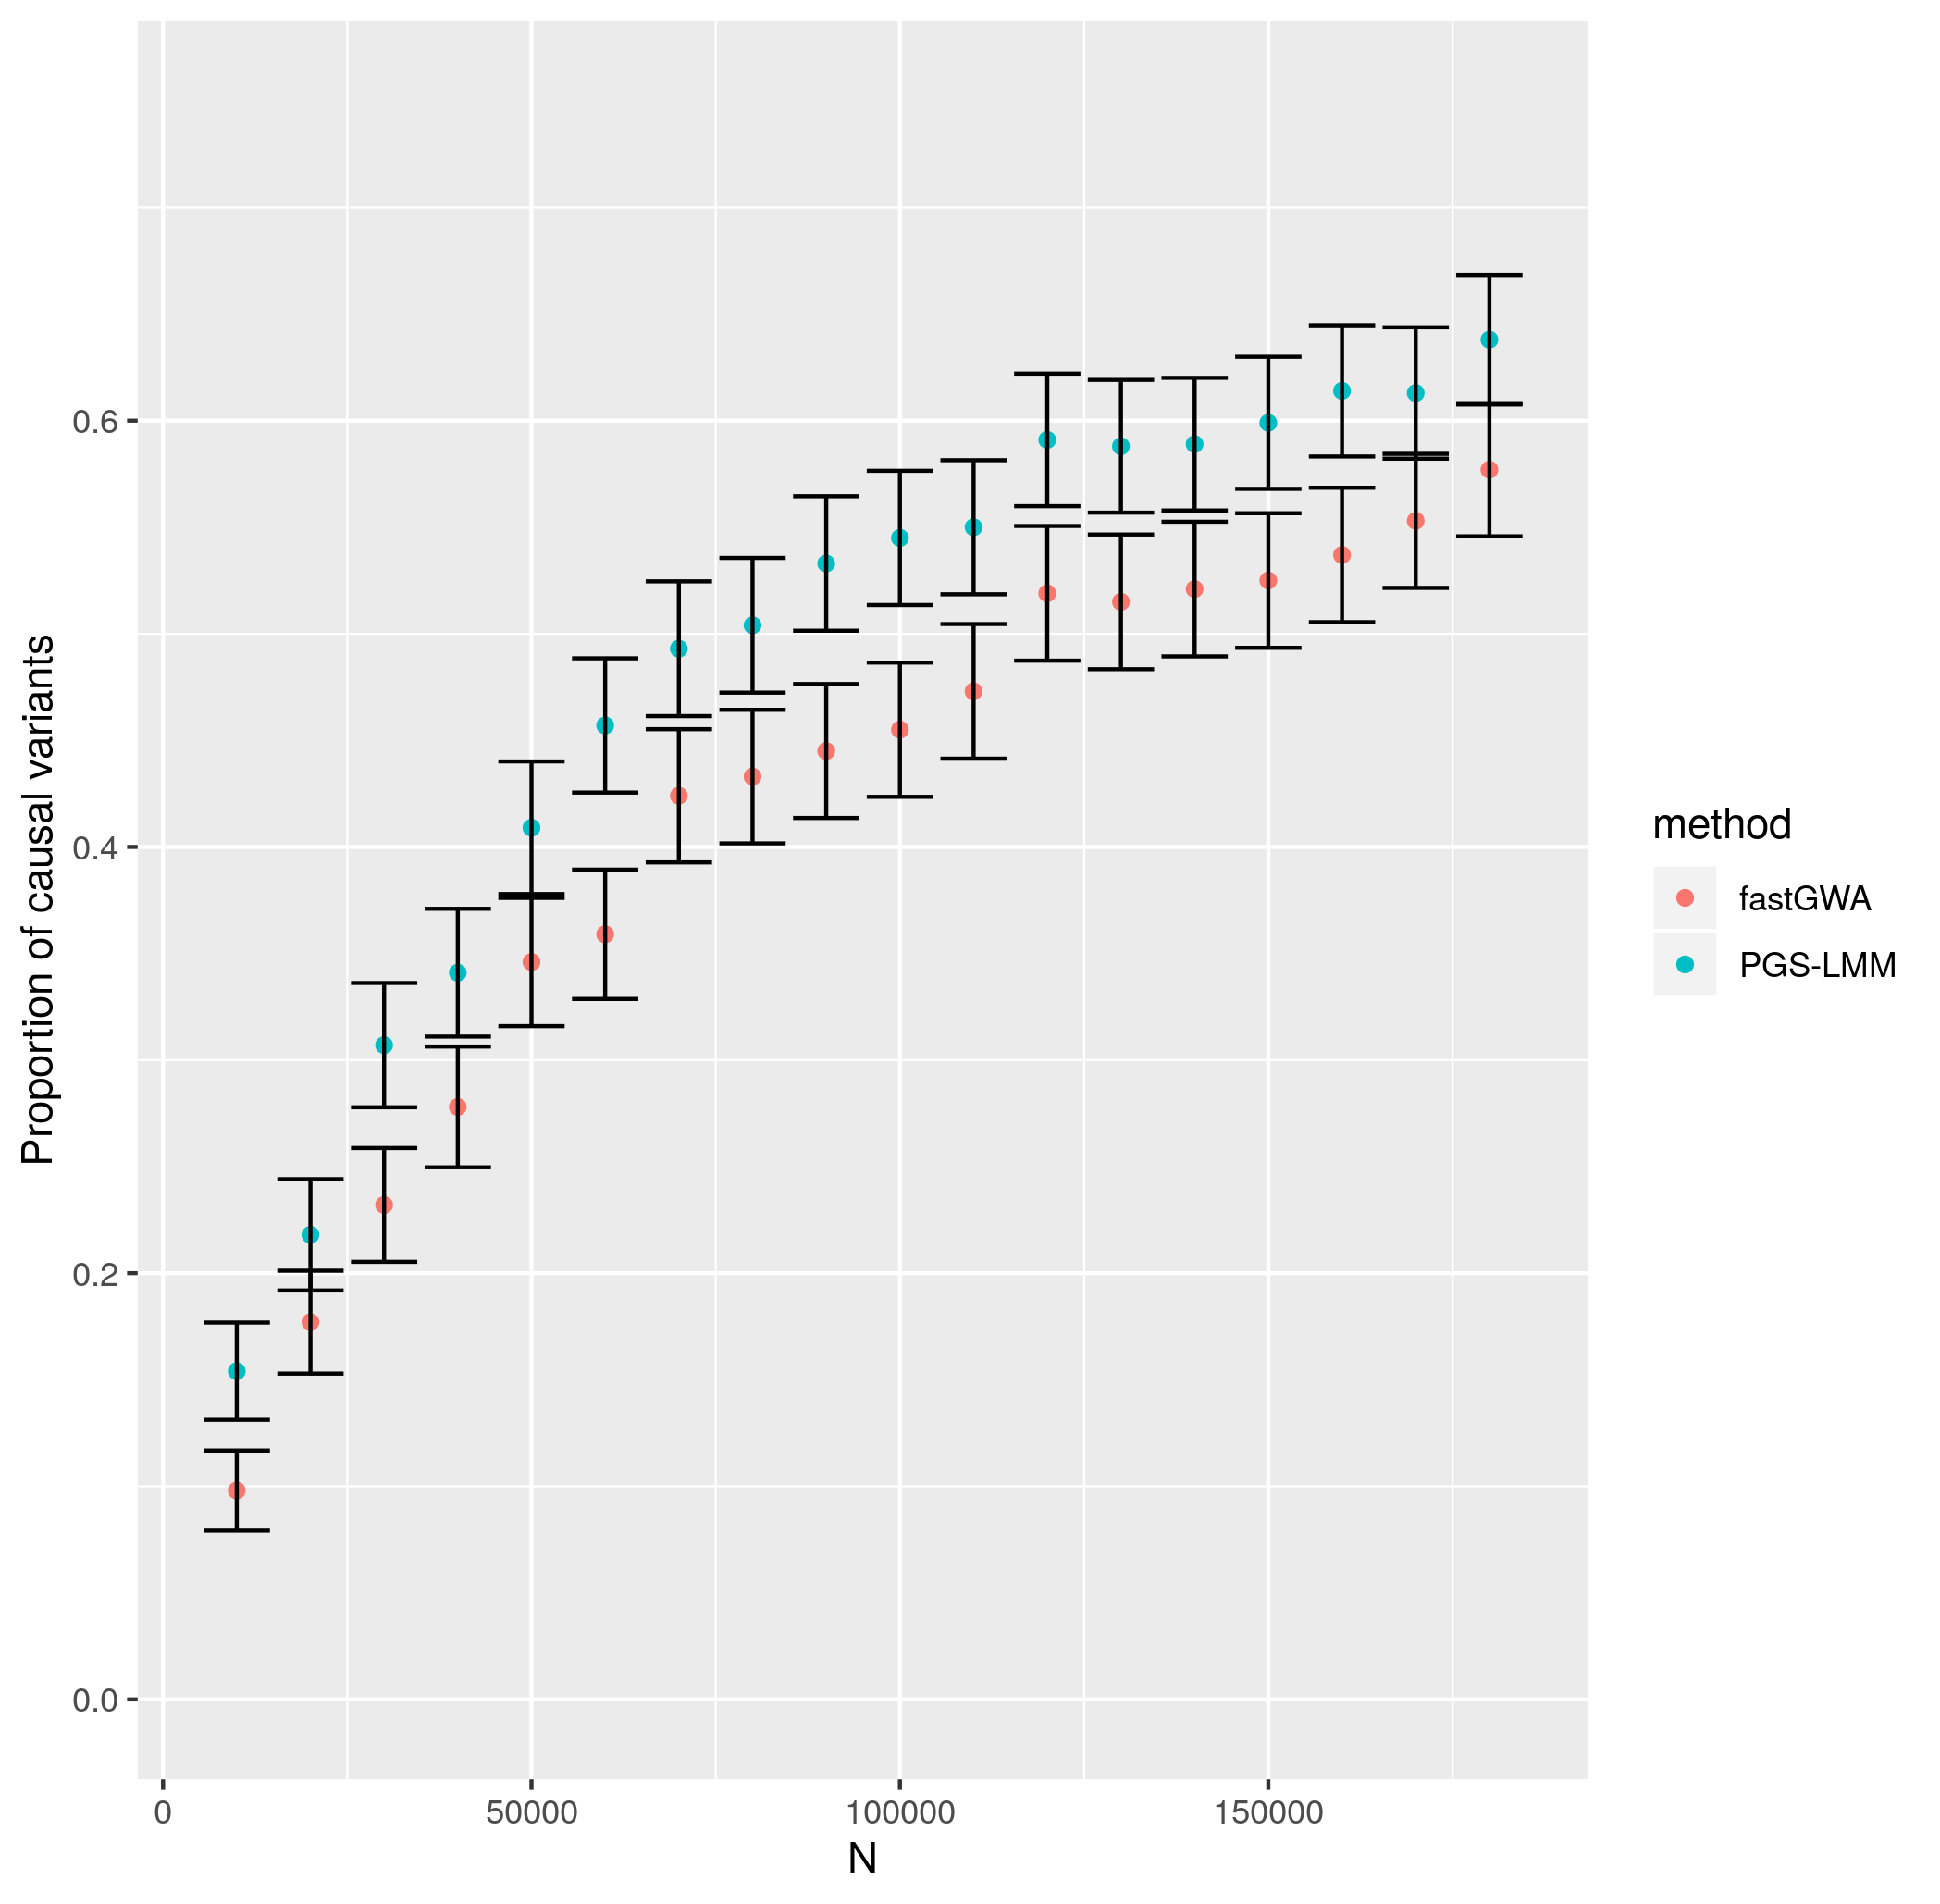
\includegraphics[width=0.85\textwidth]{images/Fig4.png}

  \caption{\csentence{Effects of sample size on PGS-LMM.}
      Proportion of causal variants identified as a function of sample size.}
      \end{figure}
      
\begin{figure}[h!]
  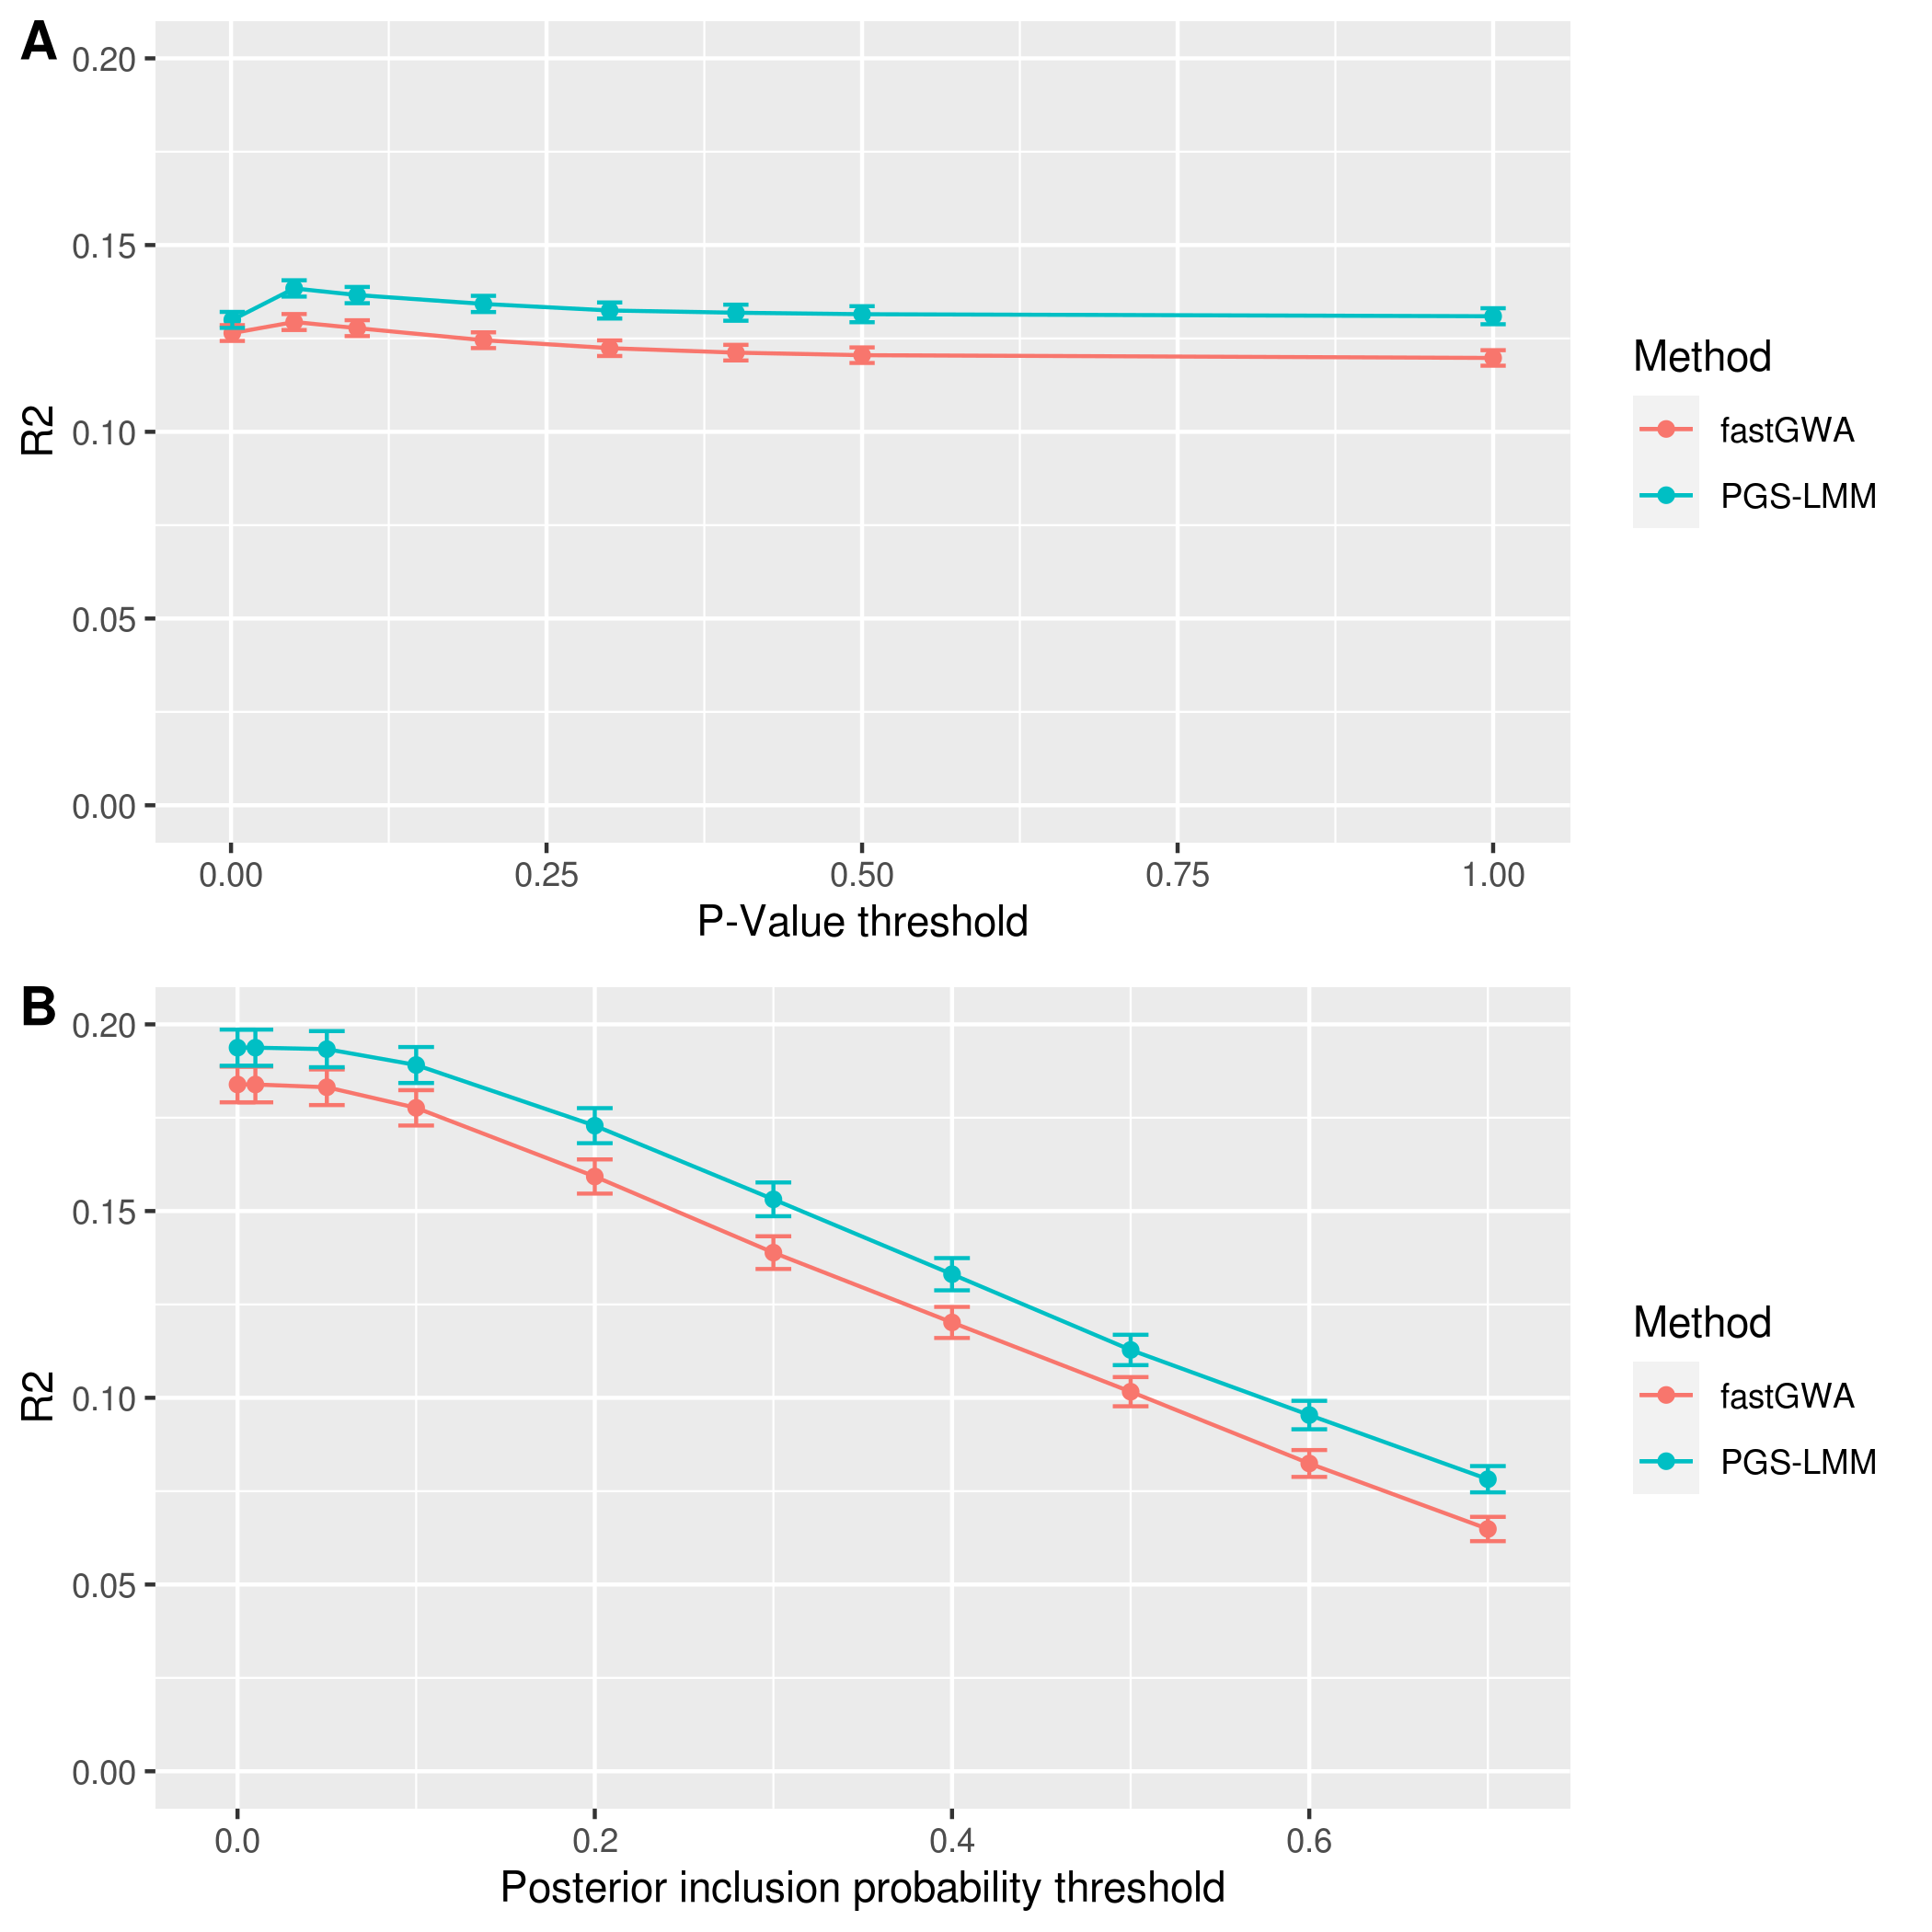
\includegraphics[width=0.85\textwidth]{images/Fig5.png}
  \caption{\csentence{PGS-LMM prediction analysis}
      P+T prediction (A) across range of p value thresholds for each method Bayesian inference prediction (B) across PIP scores. Summary statistics are calculated on the 80\% training data}
      \end{figure}

%%%%%%%%%%%%%%%%%%%%%%%%%%%%%%%%%%%
%%                               %%
%% Tables                        %%
%%                               %%
%%%%%%%%%%%%%%%%%%%%%%%%%%%%%%%%%%%

%% Use of \listoftables is discouraged.
%%
%\section*{Tables}
%\begin{table}[h!]
%\caption{Sample table title. This is where the description of the table should go.}
%      \begin{tabular}{cccc}
%        \hline
%           & B1  &B2   & B3\\ \hline
%        A1 & 0.1 & 0.2 & 0.3\\
%        A2 & ... & ..  & .\\
%       A3 & ..  & .   & .\\ \hline
%      \end{tabular}
%\end{table}

%%%%%%%%%%%%%%%%%%%%%%%%%%%%%%%%%%%
%%                               %%
%% Additional Files              %%
%%                               %%
%%%%%%%%%%%%%%%%%%%%%%%%%%%%%%%%%%%

\section*{Additional Files}
  \subsection*{Additional file 1 --- Sample additional file title}
    PDF file of supplementary figures S1-S6 and supplementary tables 1-3.

%  \subsection*{Additional file 2 --- Sample additional file title}
%    Additional file descriptions text.


\end{backmatter}
\end{document}
